\documentclass[times, 10pt,twocolumn]{article} 
\usepackage{latex8}
\usepackage{times}

\pagestyle{empty}

\usepackage{amsmath}
\usepackage{fullpage}
\usepackage{epsfig}
\usepackage{subfigure}
\usepackage{setspace}
%%%%%%%%%%%%%%%%%%%%%%%%%%%%%%%%%%%%%%%%%%%%%%%%%%%%%%%%%%%%%%%%%%%%%%
%%%%%%%%%%%%%%%%%%%%%%%%%%%%%%%%%%%%%%%%%%%%%%%%%%%%%%%%%%%%%%%%%%%%%%
%%%%%%%%%%%%%%%%%%%%%%%%%%%%%%%%%%%%%%%%%%%%%%%%%%%%%%%%%%%%%%%%%%%%%%

\begin{document}

\title {\bf A Productive Programming Environment for Stream Computing}

\author{
  Kimberly Kuo, Rodric M. Rabbah, Saman Amarasinghe\\
  Computer Science and Artificial Intelligence Laboratory\\
  Massachusetts Institute of Technology\\
  Cambridge, MA 02139\\
  \{kkuo, rabbah, saman\}@csail.mit.edu
}

\maketitle
\thispagestyle{empty}

\begin{abstract}
This paper  presents StreamIt and  the StreamIt Development  Tool. The
development tool is an IDE  designed to improve the coding, debugging,
and visualization of streaming  applications by exploiting the ability
of  the StreamIt language  to naturally  represent streaming  codes as
structured, hierarchical  graphs.  The StreamIt  Development Tool aims
to emulate  the best  of traditional debuggers  and IDEs  while moving
toward hierarchical  visualization and debugging  concepts specialized
for streaming applications.  As such, it provides utilities for stream
graph  examination,  tracking  of   data  flow  between  streams,  and
deterministic  execution of  parallel streams.  These features  are in
addition to  more conventional tools  for creating and  editing codes,
integrated   compilers,    setting   breakpoints,   watchpoints,   and
step-by-step program execution.

A user study evaluating StreamIt  and the development tool was held at
MIT during which participants  were given erroneous programs and asked
to resolve  the programming errors.   We compared the  productivity of
the users when  using the StreamIt Development Tool  and its graphical
features  to  those who  were  restricted  to line-oriented  debugging
strategies, and  we found  that the former  produced ten  more correct
solutions compared to  the latter set of users.  Furthermore, our data
suggests  that  the  graphical  tool  chain helped  to  mitigate  user
frustration and  encouraged participants to invest  more time tracking
and fixing programming errors.
\end{abstract}

%%%%%%%%%%%%%%%%%%%%%%%%%%%%%%%%%%%%%%%%%%%%%%%%%%%%%%%%%%%%%%%%%%%%%%
%%%%%%%%%%%%%%%%%%%%%%%%%%%%%%%%%%%%%%%%%%%%%%%%%%%%%%%%%%%%%%%%%%%%%%
%%%%%%%%%%%%%%%%%%%%%%%%%%%%%%%%%%%%%%%%%%%%%%%%%%%%%%%%%%%%%%%%%%%%%%

\section{Introduction}

The last  few years  have witnessed the  rebirth of  supercomputing as
computer  scientists  and engineers  realize  that current  monolithic
architectures and  conventional von~Neumann programming  styles are at
their  limits in  terms of  deliverable performance  to  the end-user.
Thus  as architects,  compiler engineers,  and  application developers
look  into  the  future,  there  is  a  concerted  effort  to  develop
processors  and programming paradigms  that can  deliver significantly
better  performance, and  more so,  to deliver  high  performance more
productively.  This  is especially  important since the  complexity of
applications  continues to  increase, and  compilers are  more heavily
burdened with the extraction  of parallelism and the efficient mapping
of  computation  to  physical  substrate.   What's more  is  that  the
architectures of the future  will tend toward distributed resources in
an effort  to manage the complexity of  centralized architectures with
respect to power  and wire delay. Thus, research  labs in industry and
academia alike  are investigating  ideas and methodologies  to address
the computing challenges  of the future with an  eye toward delivering
high performance  and to do  so productively. This goal  translates to
$(i)$ relieving application  developers from architecture details and
allowing for natural expression  of applications, $(ii)$ lessening the
burden  for   heroic  compilers  that   extract  parallelism,  $(iii)$
developing  scalable architectures  that  are powerful  yet easier  to
verify and assemble.

The Computer Architecture Group at  MIT has for the last several years
conducted  research to  address all  of the  aforementioned objectives.
This   paper    focuses   on   the    productivity   of   application
developers.   Specifically,   the    paper   will   briefly   describe
StreamIt~\cite{streamitcc}  a   novel  language  for   the  prevalent
application  class of stream  computing. StreamIt  provides high-level
stream abstractions  that improve programmer  productivity and program
robustness.  The language is architecture independent, and it features
several  characteristics  (such  as parameterization  and  modularity)
geared  toward  large scale  program  development.  Furthermore,  this
paper  will  also  describe  a  unique  development  environment  that
leverages the language  features to deliver a tool chain  for the rapid
verification and debugging of StreamIt programs.

StreamIt represents  a program as  a hierarchical graph  of concurrent
filters  that operate  on streams  of  data and  communicate via  FIFO
queues.    The  language  exposes   the     parallelism  and
communication patterns  that are  inherent in many  streaming programs
which   include   software   radio,  real-time   encryption,   network
processing, graphics, and multimedia editing consoles.  Because of the
abundance  of parallelism  in such  applications, they  are especially
challenging  to program,  and worse,  to debug.   This is  due  to the
multitude of factors that  an application developer must consider when
implementing a streaming  program, such as for example  how to exploit
the   parallelism  on   a  target   architecture.   The   marriage  of
implementation  to a  specific processor  results in  both algorithmic
changes and  code transformations that  make porting difficult---since
the transformations depend on the architecture details.

By contrast, application developers  using StreamIt focus on specifying
the functional behavior of their programs and verify correctness using
high   level  abstractions   that   result  in   clean  and   portable
implementations.   The task  of  optimizing the  code and  efficiently
mapping  it to target  processors is  left to  the compiler  which can
automate many  powerful domain specific optimizations  to deliver high
performance~\cite{linear, streambit}. This  paper will not discuss the
StreamIt  compiler technology;  the  interested reader  can visit  the
StreamIt  web  page~\cite{streamit-web} for  more  information on  the
topic.

In addition  to the language  and compiler effort, we  have engineered
and  developed a programming  environment that  graphically represents
the  hierarchical nature  of streaming  codes with  an eye  toward the
productivity  of the application  engineer.  The  StreamIt Development
Tool (SDT) provides an elaborate prototyping and debugging environment
that can  interpret and visually represent  streaming computation. The
key distinguishing  features of the SDT  are its ability  to track the
flow  of data  between  streams, and  the  deterministic execution  of
parallel streams. The latter leverages an intuitive concept of time in
StreamIt that is  tied to the flow of data  in distributed programs. A
significant portion of  this paper is dedicated to  evaluating the SDT
and  its   impact  on  programmer   productivity.  Toward  quantifying
productivity, we organized  a user study at MIT.  The study involved a
number of students who were  given a set of ``buggy'' applications and
asked  to   fix  the  codes  according   to  corresponding  functional
specifications. Some of the study participants were allowed to use the
graphical  debugger and  its distinguishing  features,  whereas others
were restricted to line-oriented  debugging strategies. The results of
our study  provide evidence that  the SDT was instrumental  in helping
the users  track down and  repair programming errors. The  evidence is
particularly strong  in cases where the applications  were large, with
many streams and non trivial communication topologies.

As  we analyzed  the data  from  the user  study, we  made a  somewhat
surprising observation.   First, it was  evident that the SDT  did not
make users faster. In fact, the mean time to solution (i.e., a program
where all of the bugs are fixed) was longer for participants using the
graphical  debugger.   Perhaps  this  is  to  be  expected  since  the
participants did  not have prior  experience with the language  or the
IDE, and  indeed our post-study  interviews and feedback  support this
theory. Second,  the data suggested  that the power  of the SDT  is in
mitigating the  frustration factor of the  participants, especially in
the later portions  of the study.  That is,  the participants who were
restricted to  line-oriented debugging strategies gave  up more often,
and did so sooner, compared  to their counterparts using the graphical
debugger.   This  led  us to  conclude  that  users  tend to  be  more
productive  when they  trust the  tools  at their  disposal. In  other
words, one  might believe their  probability of success  is reasonably
high if they are confident that the tools they are using are adequate,
and therefore they are more likely to invest their time objectively.

In  the  following  Section   we  describe  the  StreamIt  programming
language,  and  in   Section~\ref{sec:de}  we  describe  the  StreamIt
development environment. Section~\ref{sec:ps} describes our user study
and reports our  results and analysis. Section~\ref{sec:rw} summarizes
related work and Section~\ref{sec:cr} concludes the paper.


%%%%%%%%%%%%%%%%%%%%%%%%%%%%%%%%%%%%%%%%%%%%%%%%%%%%%%%%%%%%%%%%%%%%%%
%%%%%%%%%%%%%%%%%%%%%%%%%%%%%%%%%%%%%%%%%%%%%%%%%%%%%%%%%%%%%%%%%%%%%%
%%%%%%%%%%%%%%%%%%%%%%%%%%%%%%%%%%%%%%%%%%%%%%%%%%%%%%%%%%%%%%%%%%%%%%

\section{The StreamIt Programming Language}
\label{sec:pl}

StreamIt  is   an  architecture-independent  language   for  streaming
applications.  It adopts the Cyclo-Static Dataflow~\cite{BELP96} model
of   computation   which    is   a   generalization   of   Synchronous
Dataflow~\cite{LM87-i}.  StreamIt  programs are represented  as graphs
where  nodes represent  computation and  edges  represent FIFO-ordered
communication of data over tapes.

The  basic programmable  unit in  StreamIt is  a filter.   Each filter
contains  a work  function that executes atomically,  popping (i.e.,
reading)  a fixed number  of items  from the  filter's input  tape and
pushing (i.e., writing) a fixed number of items to the filter's output
tape.  A filter  may also ``peek'' at a given index  on its input tape
without  consuming  the  item;  this  makes  it  simple  to  represent
computation over a ``sliding-window''.   The push, pop, and peek rates
are  declared as  part  of  the work  function,  thereby enabling  the
compiler    to    construct    a    static    schedule    of    filter
firings~\cite{lee87static}.

%% Each filter has a distinct address space.  A filter can store two
%% types of variables: a {\it field} and a {\it local}.  Fields are
%% declared in the scope of the filter and are preserved across
%% executions, while locals are declared inside the work function and are
%% only live within a single execution.  There is also an init function
%% which runs once at the beginning of the program and is used to
%% initialize fields.
%% \begin{figure}[t]
%% \vspace{-18pt}
%% \begin{singlespace}

%% ~~
%% \begin{minipage}{0.46in}
%% {\centering
%% \psfig{figure=pipeline.eps,width=0.46in} \\
%% }
%% \end{minipage} 
%% ~
%% \begin{minipage}{1.3in}
%% {\centering
%% \psfig{figure=splitjoin.eps,width=1.3in} \\
%% }
%% \end{minipage}
%% ~
%% \begin{minipage}{1.02in}
%% {\centering
%% \psfig{figure=feedback.eps,width=1.02in} \\
%% }
%% \end{minipage}
%% ~~~~~~~~~
%% \begin{minipage}{3in}
%% \vspace{36pt}
%% \psfig{figure=iir-pipeline.eps, width=2.33in}
%% ~~~~
%% \raisebox{12pt}{\psfig{figure=iir-pipeline2.eps, width=0.46in}}
%% \end{minipage}
%% \\ ~ \\ {\protect\small (a) A pipeline. ~~(b) A splitjoin. ~~(c) A feedbackloop.}

%% \begin{minipage}{3.5in}
%% \caption{Stream structures supported by StreamIt.
%% \protect\label{fig:structures}}
%% \end{minipage}
%% \begin{minipage}{3in}
%% \caption{Example pipeline with FIR filter.\protect\label{fig:iir-pipeline}}
%% \end{minipage}
%% \vspace{3pt}
%% \hrule
%% \vspace{3pt}
%% \end{singlespace}
%% \vspace{-12pt}
%% \end{figure}

\begin{figure}[t]
\begin{center}
  \framebox{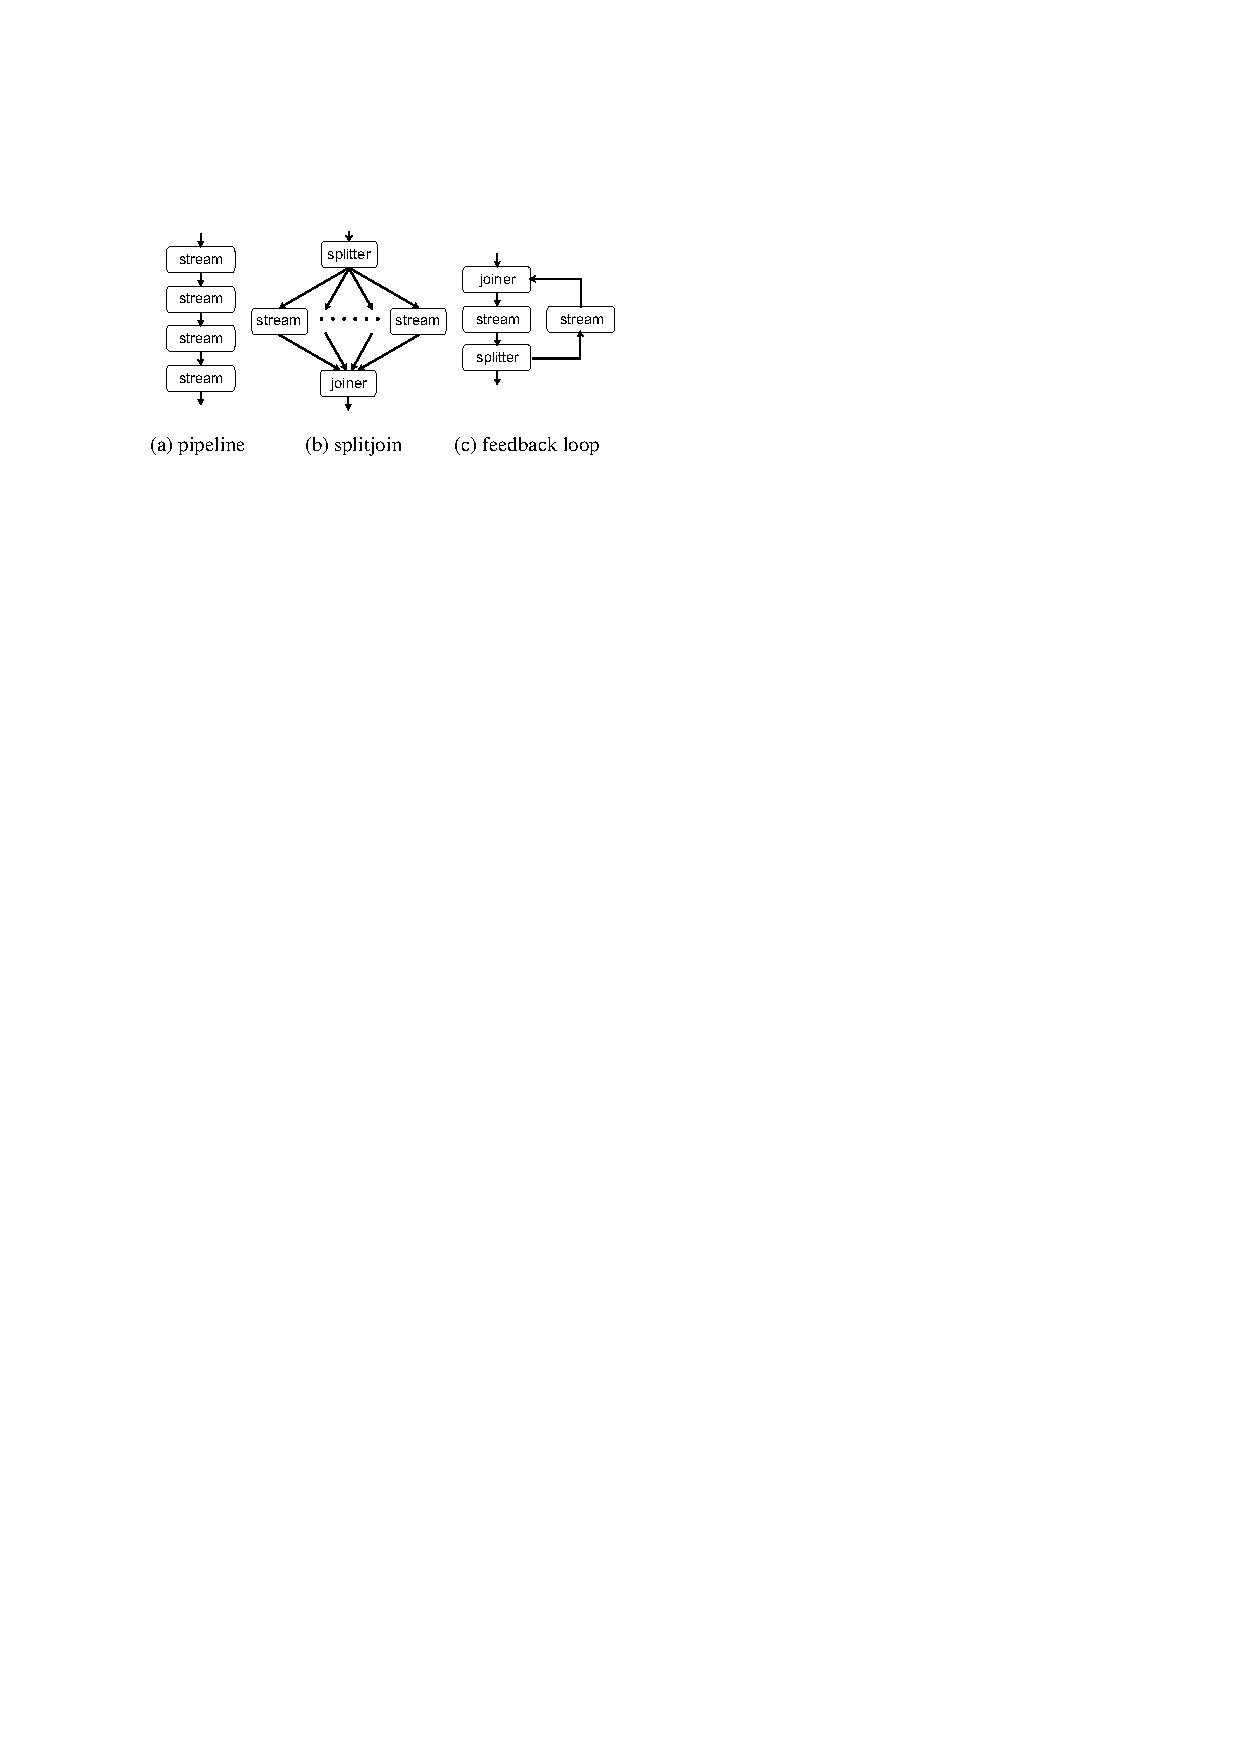
\includegraphics[scale=1, angle=0]{./constructs-eg.pdf}}
  \caption{StreamIt containers.}
  \label{fig:containers}
\end{center}
\end{figure}

\begin{figure}[t]
\begin{center}
  \framebox{\includegraphics[scale=1, angle=0]{./pipeline-eg.pdf}}
  \caption{Example pipeline with FIR filter.}
  \label{fig:pipeline}
\end{center}
\end{figure}

StreamIt provides three  hierarchical structures for composing filters
into larger stream graphs (see Figure~\ref{fig:containers}).  The {\it
pipeline} construct  composes streams in sequence, with  the output of
one connected to the input of the next.  The {\it splitjoin} construct
distributes data to  a set of parallel streams,  which are then joined
together in a round robin fashion.   The {\it feedback loop} provides a
mechanism  for introducing  cycles  in  the graph.   An  example of  a
pipeline  appears  in  Figure~\ref{fig:pipeline}.  It  contains  a
single  FIR   (Finite  Impulse   Response)  filter which   could  be
implemented as follows:
%\vspace{-0.1in}
\begin{scriptsize}
\begin{verbatim}
float->float filter FIR (int N, float[] weights) 
{
  work push 1 pop 1 peek N {
    float sum = 0;
    for (int i = 0; i < N; i++) {
      sum += peek(i) * weights[i];
    }
    pop();
    push(sum);
  }
}
\end{verbatim}
\end{scriptsize}

The filter can now serve as  a module that is incorporated into stream
graphs as necessary, for example as part of an acoustic beam former. A
filter is akin to a class in object oriented programming with the work
function  serving as  the main  method. A  filter may  also  declare a
constructor function  to initialize the filter state  before any other
method is invoked. The implementation of the work function in StreamIt
obviates  the need  for  explicit buffer  management. The  application
developer instead focuses on the  hierarchical assembly of  the stream
graph and its communication topology.

%%%%%%%%%%%%%%%%%%%%%%%%%%%%%%%%%%%%%%%%%%%%%%%%%%%%%%%%%%%%%%%%%%%%%%
%%%%%%%%%%%%%%%%%%%%%%%%%%%%%%%%%%%%%%%%%%%%%%%%%%%%%%%%%%%%%%%%%%%%%%
%%%%%%%%%%%%%%%%%%%%%%%%%%%%%%%%%%%%%%%%%%%%%%%%%%%%%%%%%%%%%%%%%%%%%%

\section{Development Environment}
\label{sec:de}

The StreamIt  Development Tool (SDT)  features many aspects of  an IDE,
including a text editor and  a debugger. For example, the SDT debugger
supports line and method breakpoints, watchpoints, program suspension,
code stepping,  variable inspection and  value modification to  list a
few.

Moreover,   the  SDT   offers  features   tailored  to   the  StreamIt
language.  The  SDT  graphically  represents  StreamIt  programs,  and
preserves hierarchical information to allow an application engineer to
focus on  the parts of  the stream program  that are of  interest. In
addition, the SDT can track the flow of data between filters, and most
importantly, it  provides a deterministic mechanism  to debug parallel
streams.

The SDT  is implemented in Java as  an Eclipse~\cite{eclipse} plug-in.
The  Eclipse universal  tools  platform is  an extensible  development
environment. We leverage the built-in user interfaces for editing and
viewing  files,  the  resource  management system,  the  documentation
infrastructure,  and the  runtime  support of  launching, running  and
debugging programs.


%%%%%%%%%%%%%%%%%%%%%%%%%%%%%%%%%%%%%%%%%%%%%%%%%%%%%%%%%%%%%%%%%%%%%%
%%%%%%%%%%%%%%%%%%%%%%%%%%%%%%%%%%%%%%%%%%%%%%%%%%%%%%%%%%%%%%%%%%%%%%

\subsection{Hierarchical Graphs}

\begin{figure*}[t]
\begin{center}
  \subfigure[Collapsed pipeline.\label{fig:eg-hierarchy-collapsed}]{
    \framebox{\includegraphics[scale=.5, angle=270]{./hierarchy-eg1.pdf}}
  }
  \subfigure[Expanded splitjoin.\label{fig:eg-hierarchy-expanded}]{
    \framebox{\includegraphics[scale=.5, angle=270]{./hierarchy-eg2.pdf}}
  }
  \subfigure[Example pipeline with data in transit.\label{fig:dataflow}]{
    \framebox{\includegraphics[scale=.5, angle=270]{./dataflow-eg.pdf}}
  }
  \caption{Hierarchical stream graph views.}
  \label{fig:hierarchy}
\end{center}
\end{figure*}

As  seen  in Figure~\ref{fig:hierarchy},  a  StreamIt  program can  be
visually depicted  as a hierarchical  directed graph of  streams, with
graph nodes representing streams and graph edges representing tapes or
channels.   The   containers  are  rendered  according   to  the  code
declarations, and the visualization tools in the SDT allow the user to
selectively collapse  and expand containers.  This is  useful in large
streams  where  the  application  developers are  only  interested  in
visualizing   a  particular   subset,  for   example  to   verify  the
interconnect       topology        of       the       graph.        In
Figure~\ref{fig:eg-hierarchy-collapsed}, we show  a screen shot of the
SDT  for a simple  StreamIt program  which consists  of a  filter that
generates input data (\texttt{IntSource}), a splitjoin (\texttt{Echo})
that operates on the data produced  by the source and whose data is in
turn    consumed   by   an    \texttt{Adder}.    Lastly,    a   filter
(\texttt{IntPrinter})  reads and  prints  the computed  values to  the
screen.   In Figure~\ref{fig:eg-hierarchy-expanded}, the  splitjoin is
expanded  to   reveal  to  parallel   streams:  \texttt{Original}  and
\texttt{Delay}. The  former is simply an identity  filter, whereas the
later shifts its input data one position in time (i.e., at time $t$ it
outputs data consumed at time $t+1$. The splitter in this example is a
duplicate splitter, meaning that the input stream is duplicated to all
of its siblings. The joiner  is a roundrobin joiner which collects one
data item  from the  left stream  followed by an  item from  the right
stream. This particular stream program simulates how echos are added
to sound waves.

%%%%%%%%%%%%%%%%%%%%%%%%%%%%%%%%%%%%%%%%%%%%%%%%%%%%%%%%%%%%%%%%%%%%%%
%%%%%%%%%%%%%%%%%%%%%%%%%%%%%%%%%%%%%%%%%%%%%%%%%%%%%%%%%%%%%%%%%%%%%%

\subsection{Data Flow}

%% \begin{figure}[t]
%% \begin{center}
%%   \framebox{\includegraphics[scale=1, angle=0]{./dataflow-eg.pdf}}
%%   \caption{Example pipeline with data in transit.}
%%   \label{fig:dataflow}
%% \end{center}
%% \end{figure}

An important distinguishing characteristic  of the SDT is its ability
to track  the flow  of data between  streams.  This is  illustrated in
Figure~\ref{fig:dataflow} which  shows the  data that is  live between
two  filters  \texttt{Source}  and \texttt{DropBit}.  This  particular
program  generates  a sequence  of  numbers  at  its source,  and  the
\texttt{DropBit} filter removes the third element of the sequence with
every execution of its main function.  In the figure, the values 2, 3,
and 4 are  queued on the input tape to  \texttt{DropBit}, and from the
expanded filter node, we can  see that the filter requires four queued
data items  before the work  function can execute (i.e.,  the declared
pop rate is 4). The expanded filter node also displays other
information such as the input and output types of the stream, as well
as profiling information that is useful for debugging.

The SDT also allows the user to highlight and automatically track data
items as  they propagate  between streams.  The  user can  also modify
values on  a tape, much like  a conventional debugger  allows users to
modify variables and registers.

The flow of data is especially helpful in splitjoins where sequential
data streams are distributed to parallel streams, and parallel streams
assembled into a single stream. The visualization allows the user to
readily  verify  that  splitters  and joiners  implement  the  desired
functionality.  Also,  the   visualization  allows  users  to  quickly
pinpoint unexpected outputs (e.g., a filter pushing NaN's).

%%%%%%%%%%%%%%%%%%%%%%%%%%%%%%%%%%%%%%%%%%%%%%%%%%%%%%%%%%%%%%%%%%%%%%
%%%%%%%%%%%%%%%%%%%%%%%%%%%%%%%%%%%%%%%%%%%%%%%%%%%%%%%%%%%%%%%%%%%%%%

\subsection{Debugging Parallel Streams}

Perhaps  the most  important feature  of the  SDT is  its  support for
debugging parallel  streams. In StreamIt,  the streams in  a splitjoin
are  independent, and can  execute when  their corresponding  data are
queued.  Thus, the SDT can execute parallel streams in a deterministic
order using  a single  program counter and  machine state; this  is in
contrast to  a multi-threaded  program where a  user has to  cope with
multiple  program counters  and  a scheduling  order  that may  appear
non-deterministic   and  subject   to  the   host   operating  system.
Furthermore, by exposing  the flow of data and  the communication in a
stream graph, StreamIt provides a  natural way to reason about time in
a  distributed  system---thereby   greatly  simplifying  the  task  of
debugging parallel streaming programs.

The SDT  also features a unique  capability that allows a  user to set
instance-breakpoints. This features is useful in splitjoins with many
parallel streams or in long pipelines which contain multiple instances
of  a  single filter.  As  with  conventional  debuggers, the  program
executes until the designated instance of a filter is encountered---in
which case control is transfered to the user for further input.


%%%%%%%%%%%%%%%%%%%%%%%%%%%%%%%%%%%%%%%%%%%%%%%%%%%%%%%%%%%%%%%%%%%%%%
%%%%%%%%%%%%%%%%%%%%%%%%%%%%%%%%%%%%%%%%%%%%%%%%%%%%%%%%%%%%%%%%%%%%%%
%%%%%%%%%%%%%%%%%%%%%%%%%%%%%%%%%%%%%%%%%%%%%%%%%%%%%%%%%%%%%%%%%%%%%%

\section{Productivity Study}
\label{sec:ps}

We designed and carried out a  user study to assess the extent the SDT
helps in debugging StreamIt programs.  The goals were two fold. First,
we aimed to identify difficulties in using the SDT and toward this end
we used questionnaires and  automatic action logging.  The second goal
was to gather data to support  the hypothesis that the SDT can improve
a programmer's ability to debug StreamIt applications.

We provided  participants with a  set of ``buggy''  StreamIt programs,
along with verbal descriptions of the programs.  The participants were
asked to find and fix the  errors and to record their experience using
various forms  and questionnaires.  The participants  were divided into
different  groups,  some of  which  used  the  SDT and  its  graphical
debugging features  whereas others did not.  Our  results and analysis
are reported  in the  following sections.

%%%%%%%%%%%%%%%%%%%%%%%%%%%%%%%%%%%%%%%%%%%%%%%%%%%%%%%%%%%%%%%%%%%%%%
%%%%%%%%%%%%%%%%%%%%%%%%%%%%%%%%%%%%%%%%%%%%%%%%%%%%%%%%%%%%%%%%%%%%%%

\subsection{Target Population}

We solicited participants for the  user study by advertising it to MIT
students  majoring  in  computer  science.  We  favored  students  who
specialize in communications,  signal processing, computer systems and
architecture, and who are  experienced in popular imperative languages
(e.g., C, C++, Java).  The nature of study was not explicitly divulged
in  our solicitation;  this  served to  prevent  potential users  from
learning about  StreamIt and becoming  familiar with the SDT  prior to
the  study. The  participants were  awarded a  small monetary  gift upon
completion of the study.

%%%%%%%%%%%%%%%%%%%%%%%%%%%%%%%%%%%%%%%%%%%%%%%%%%%%%%%%%%%%%%%%%%%%%%
%%%%%%%%%%%%%%%%%%%%%%%%%%%%%%%%%%%%%%%%%%%%%%%%%%%%%%%%%%%%%%%%%%%%%%

\subsection{Methodology}

Each participant in the user study was presented with a  set of
documents that described the tasks of the study and which served to
record information from the participants during the study. The
documents were:
\begin{enumerate}
\item Pre-Study  Questionnaire: This  document was designed  to gather
information  on  the participant's  programming  background and  skill
level. Questions such  as year in school, major,  degree being sought,
area  of computer  science concentration,  relevant  classes, language
proficiency,  application development  experience,  and background  in
DSP, IDE, and the SDT were asked.
\item  StreamIt  Language  Tutorial:  This  written  presentation  was
intended to give  a cursory introduction to the  StreamIt language. It
described  and illustrated the  syntax and  semantics of  the StreamIt
language. Furthermore,  example toy applications and tips  on the most
common  mistakes new  StreamIt  programmers are  likely  to make  were
included.
\item SDT  Tutorial: Another  written presentation, this  document was
aimed at  informing users  of the essential  features of the  SDT. The
first part of the tutorial described the functionality of the StreamIt
editor  and  debugger.  The  second  part of  the  document  contained
step-by-step instructions on  how to compile, run, and  debug a sample
application.
\item  User  Tasks:  This  document  instructed users  to  debug  nine
StreamIt applications in  a specific order. Each of  the nine programs
contained one  or more bugs.  As  the users moved from  one program to
the next,  they were asked  to record their  start and end  times, the
debugging methods they used  (e.g., code inspection, print statements,
graphical debugger),  and a short  diagnosis of the program  bugs they
uncovered.
\item Description of Applications  and Code: This document contained a
description  of  each  application  (numbered  1 through  9),  a  code
listing, a sample buggy output, and a sample correct output. The
applications are summarized in Table~\ref{tab:applications}.
\item Post-Study  Questionnaire: This document was  designed to gather
data pertaining to the participant's experience, such as the perceived
difficulty  of each  problem, a  general description  of how  the user
debugged  each application,  user satisfaction,  ability to  learn and
recall various features of the SDT, etc.
\end{enumerate}

\begin{table*}
\caption{Applications used in the productivity study.}
\centering
\begin{tabular}{|l|p{5.0in}|} \hline
\label{tab:applications}
{\bf 1. Bit Twiddle} & Removes every third bit from a 96 bit stream.\\ \hline
{\bf 2. Fib}         & Generates a Fibonacci sequence using a feedback loop.\\ \hline
{\bf 3. Echo Effect} & Simulates how echos are introduced into sound waves. Uses a splitjoin with two parallel streams.\\ \hline
{\bf 4. Merge Sort}  & Implements a merge sort algorithm using 16 parallel streams.\\ \hline
{\bf 5. Cornerturn}  & Implements a matrix transpose using a splitjoin to exchange the rows and columns. Stresses the visual tracking of data.\\ \hline
{\bf 6. Echo Effect2}& Alternate implementation of Echo Effect using a feedback loop.\\ \hline
{\bf 7. Bubble Sort} & Implements a bubble sort algorithm. This is a conceptually difficult implementation that stresses the visualization features of the debugger.\\ \hline
{\bf 8. Bit Reverse} & Sorts a sequence of 16 consecutive numbers in bit-reversed order. This is an adaptation of the bit-reversal stage in FFT.\\ \hline
{\bf 9. Overflow}  & A synthetic benchmark with a substantial number of hierarchies, filters, and parallel streams. Stresses the visual tracking of data, and the instance breakpoint capabilities of the debugger.\\ \hline
\end{tabular}
\end{table*}

In  order  to minimize  biased  effects  on  a programmer's  debugging
ability, and to ensure internal validity, users were grouped into four
categories.  All users  were asked to debug application  1 without the
SDT's graphical  features. The participants  were then asked  to debug
application  2  using  the  SDT  and  its  graphical  features.  These
``control''  experiments served  to  create a  baseline reference  for
meaningful comparison later on\footnote{The control experiments served
mainly to filter data. We  did not use data attributed to participants
who  did  not  complete  the control  experiments.}.   Moreover,  the
control   applications   were   designed   to   bolster   the   user's
confidence.  Next, half  of the  users (group  A) were  told  to debug
applications 3, 4, and 5 with the  SDT and 6, 7, and 8 without the SDT
(i.e.,  using the  graphical  features  of the  SDT  then without  the
graphical features). Meanwhile, the other  half (group B) were told to
debug 3, 4, and  5 without the SDT and 6, 7, and  8 with the SDT.  Due
to this grouping structure, applications 3 and 6, 4 and 7, and 5 and 8
were designed to be of comparable difficulty.  For application 9, half
of group A (A1) and half of  group B (B1) were asked to debug with the
SDT, while  the other halves (A2  and B2) were asked  to debug without
the SDT.   Cross-sectioning the groups was aimed  at ensuring external
validity.

The study was divided into three sessions over a three-day period.  We
estimated that each session would  last for two hours (with 45 minutes
spent  on  the  tutorials  and  the  rest of  the  time  dedicated  to
debugging), but  in reality  the sessions spanned  an average  of four
hours.  Many users  were either unable or did not  have enough time to
debug certain  applications.  Participants were asked  to complete the
set of  documents at  their own pace,  and upon completion,  they were
individually interviewed and received a \$40 gift certificate.  During
the study, users were encouraged to ask questions although particulars
relating to the problems and the SDT were not revealed.

%%%%%%%%%%%%%%%%%%%%%%%%%%%%%%%%%%%%%%%%%%%%%%%%%%%%%%%%%%%%%%%%%%%%%%
%%%%%%%%%%%%%%%%%%%%%%%%%%%%%%%%%%%%%%%%%%%%%%%%%%%%%%%%%%%%%%%%%%%%%%

\subsection{Results and Analysis}

Even though 25  users were  scheduled  to participate  (5 people  for
sessions 1 and  2 and 15 people for  session 3), cancellations reduced
the participation to 20 users  and led to uneven groupings. There were
6 people in A1, 5 in A2, 4 in B1, and 5 in B2. Of the 20 participants,
there were 4 juniors, 2 seniors,  8 masters, and 6 Ph.D. students, all
majoring in Electrical Engineering and Computer Science. None of the
users had prior StreamIt or SDT experience.

\begin{figure*}[t]
\begin{center}
  \includegraphics[scale=.70, angle=270]{./users-results.pdf}
  \caption{Summary of results.}
  \label{fig:solutions}
\end{center}
\end{figure*}

Figure~\ref{fig:solutions} summarizes the study in terms of the number
of solutions  reported for each of  the applications in  the study. In
the figure,  the bars  labeled ``solved with  the SDT''  represent the
number   of  participants  that   fully  debugged   the  corresponding
applications using the SDT and its graphical features.  Similarly, the
bars  labeled  ``solved without  the  SDT''  represent  the number  of
participants  that  fully   debugged  the  corresponding  applications
without  using  the graphical  debugger.  The  bars  that are  labeled
``unsolved'' represent  the number of  participants whose applications
remained buggy.  For example, for  the application \texttt{EchoEffect}
there were two users who were  allowed to used the SDT and were unable
to debug the  code properly. There was also  one other participant who
did not  debug \texttt{EchoEffect} although this user  was not allowed
to use the SDT's graphical features.

Because the groupings are  uneven as previously mentioned, the numbers
seen in  the figure are weighted  depending on which  group is lacking
users. The  percentage above each quadruple of  columns represents the
percentage increase  or decrease in  debugged applications due  to the
SDT (and its graphical features).  For example, the graphical debugger
did not particularly help in applications 3, 4, and 5, but did help in
debugging  the  others.  On  average,  1.56  fewer participants  fully
debugged applications 3,  4, and 5 when using  the graphical debugger,
and 2.56  more users debugged applications  6, 7, 8, and  9 when using
the graphical debugger.

\begin{figure*}[t]
\begin{center}
  \includegraphics[scale=.70, angle=270]{./times-results.pdf}
  \caption{Summary of results.}
  \label{fig:times}
\end{center}
\end{figure*}

Figure~\ref{fig:times} compares the  average time spent debugging each
application. The  percentage above each set of  columns represents the
percentage improvement or deficiency in  time caused by using the SDT.
On  average,   users  took  7.78  (36.48\%)  more   minutes  to  debug
applications 3, 4, 5, 6, 7, and 9 when using the graphical features of
the  debugger,   compared  to  participants   using  more  traditional
debugging means. Furthermore, participants who were allowed to use the
SDT and its graphical features  spent an average of 16.96 more minutes
debugging applications  6, 7,  and 8, compared  to an average  of 10.67
minutes invested by  the participants who could not  use the graphical
debugger. In  both cases  the participants did  not fully  debug their
respective applications.

Summarizing the results, we found  that more participants were able to
successfully  debug their  applications  when using  the  SDT and  its
graphical features.  However, we  also observed that the SDT increased
the  ``time to  solution'' as  users had  to navigate  through  a user
interface  they were  not familiar  with. Interestingly,  we  can also
observe that  the SDT may  have mitigated user frustration.   As noted
earlier, users generally  spent much more than the  two hours allotted
to complete  the study, and as  such, users became  frustrated and may
have rushed  with the later applications.  Correspondingly, this might
have caused users  to spend less time and  debug fewer applications as
users progressed through the study.  Although this pattern is true for
participants  who  did  not  use  the SDT,  the  opposite  occurs  for
participants who used  the SDT: 41.76\% more users  were able to debug
applications 6,  7, 8, and 9  using the SDT.  Furthermore, users spent
83.35\% more time tracking down bugs  in applications 6, 7, and 8 when
using the  graphical debugger.  These  results suggest that  users are
willing to spend more time and work on more problems when using a tool
that they felt more certain would lead them to a solution.

%%%%%%%%%%%%%%%%%%%%%%%%%%%%%%%%%%%%%%%%%%%%%%%%%%%%%%%%%%%%%%%%%%%%%%
%%%%%%%%%%%%%%%%%%%%%%%%%%%%%%%%%%%%%%%%%%%%%%%%%%%%%%%%%%%%%%%%%%%%%%

\subsection{User Feedback}

Comments  obtained  from  the  post-study  questionnaires  were  quite
helpful  toward   finding  new   feature  ideas  and   problems  with
functionality, performance, reliability, and usability.

Summarizing  the most  notable  feedback, users  largely commented  on
their difficulties using Eclipse and navigating the StreamIt code. Ten
participants reported that  the time alloted to learn  how to navigate
Eclipse was too  short, and that the many  windows, menus, and options
made   it  difficult   to  find   vital  information   quickly.   Five
participants  noted that  they were  uncomfortable or  unaccustomed to
thinking  in terms  filters and  streams, while  an equal  number also
found  it overwhelming  to remember  some of  the language  syntax and
concepts.

In general however, participants rated the SDT a 3.85 on average (on a
scale of  1 to 10,  from easy to  hard), praising many aspects  of the
stream  graph viewer (e.g.,  hierarchical representation).   Those who
rated  the  SDT as  helpful,  stressed that  it  was  most useful  for
graphically visualizing  the flow of data in  the programs, especially
when the applications were large.

%%%%%%%%%%%%%%%%%%%%%%%%%%%%%%%%%%%%%%%%%%%%%%%%%%%%%%%%%%%%%%%%%%%%%%
%%%%%%%%%%%%%%%%%%%%%%%%%%%%%%%%%%%%%%%%%%%%%%%%%%%%%%%%%%%%%%%%%%%%%%

\subsection{Discussion}

Many problems and issues arose in running the study itself. One of the
major  problems  was the  time  allotted  for  users to  complete  the
study.  As previously  mentioned,  the slowest  user  spent twice  the
budgeted  amount of  time.  The  timing negatively  impacted  users in
several  ways, all of  which contributed  to incomplete  or unreliable
data:  Users  became  frustrated  and  overwhelmed by  the  amount  of
information presented to them; Users were unable to complete the study
due  to  time  constraints;  Users  did  not  properly  fill  out  the
post-study questionnaire, etc.

We  believe that  better screening  can  help bridge  the gap  between
between participants, although the biggest lesson learned centers on the
method of compensating  the participants.  Specifically, a multi-level
pay  scale for  compensation may  have  alleviated some  of the  above
problems and lead to more conclusive results. A graded pay scale would
allow each  participant to  judge whether they  can or are  willing to
complete the study. In other words, each user is rewarded according to
their   investments.    Nonetheless,   the   expertise   gap   between
participants  in a user  study is  a well-documented  issue: Usability
studies have found that the best users are often ten times better than
the worst users,  and the fastest quartile of users  are twice as fast
as   the  slowest   quartile   of  users~\cite{controlled-experiments,
research-issues}.  However, because increasing  the number of users in
a study only narrows the standard  deviation of the mean by the square
root   of  the   number  of   users\cite{controlled-experiments},  the
improvement  in  results  and  reliability  becomes  an  expensive  and
time-consuming task.   For example, in  order to double  accuracy, the
number of participants in this study would have to be quadrupled to 80
users, which would cost an additional \$2400 and 24 man-hours.

%% In  the   post-study
%% questionnaire, several users commented  that they were unaccustomed to
%% thinking  in terms of  streaming applications,  while some  users made
%% remarks  that  suggested they  never  truly  understood how  streaming
%% applications  work. In  general, the  more inexperienced  users either
%% focused  their  attentions on  Eclipse-related  and StreamIt  language
%% problems, indicating  a lack of IDE  and language-learning experience,
%% or  relied almost  exclusively on  breakpoint functionality  and print
%% statements. Because several of  the applications were designed to test
%% the effectiveness  of the graphical debugger, these  applications were
%% purposely  written   to  be  too  large  and   complicated  for  these
%% traditional debugging techniques.

%%%%%%%%%%%%%%%%%%%%%%%%%%%%%%%%%%%%%%%%%%%%%%%%%%%%%%%%%%%%%%%%%%%%%%
%%%%%%%%%%%%%%%%%%%%%%%%%%%%%%%%%%%%%%%%%%%%%%%%%%%%%%%%%%%%%%%%%%%%%%
%%%%%%%%%%%%%%%%%%%%%%%%%%%%%%%%%%%%%%%%%%%%%%%%%%%%%%%%%%%%%%%%%%%%%%

\section{Related Work}
\label{sec:rw}

%~\cite{42,35,7,39,19,6,9,36}
Numerous  debuggers  and program  visualization  tools  exist for  DSP
applications  written in C/C++  and assembly.   The majority  of these
tools   are  targeted   at  specific   hardware   platforms,  offering
traditional debugging  features (i.e., program  suspension, breakpoint
stepping,  watchpoints,  local  variable  and  output  display,  etc.)
combined with assembly code, memory register, and signal plot display.

In recent years,  some movement in the streaming  domain has been made
toward  OOP   languages  such  as   C++  or  Java,   which  introduce
abstractions   that  improve  the   portability  and   reusability  of
code. The  introduction of conceptual  abstractions empowers
the design,  debugging, visualization, and analysis  tools created for
OOP  based streaming applications  to introduce  hierarchical, modular
structures while  hiding unnecessary  details from the  programmer. On
top of  the traditional  debugging features previously  mentioned, all
three of the  tools described next use some variation  on the theme of
signal processing blocks that  are connected, displayed, and navigated
graphically.

Simulink  is a  modeling, simulation,  and analysis  tool for
control,  signal processing,  and communications  system  design. This
tool  imposes   OOP  conventions  on  Matlab,  C,   Fortran,  and  Ada
programmers  by allowing  its  users  to insert  their  code into  the
methods of pre-defined blocks  or to use application-specific standard
block libraries. Furthermore,  hierarchically block navigation at both
the  design and  debugging  stages is  offered: command-line  Simulink
Debugger enables breakpoint stepping of the currently executing method
which is simultaneously displayed on its associated block.  Additional
information, such as block state,  inputs, and outputs, are visible in
other windows.

Process-Level  Debugger  (PDG) is  designed  for a  graphical
parallel  programming environment  for concurrent  applications called
GRAPE. The PDG models processes as black boxes that interact with each
other. Like Simulink, programmers build their applications by creating
and connecting black boxes hierarchically (i.e., each black box may be
composed  of  sub-boxes--subprocesses--and  displayed in  a  graphical
view). As an application is  debugged, the PDG shows the application's
behavior  in  a  window  and  allows  a programmer  to  zoom  down  on
suspicious process  blocks in the hierarchy.   This top-down debugging
method can eventually find the associated erroneous code.

The MULTI Integrated Development Environment is designed for
multiprocessor, distributed systems and embedded applications using C,
C++,  Ada,  Fortran,  and   assembly.  Besides  standard  editing  and
debugging functionality,  this IDE  conveys program control  flow with
perusable  static and dynamic  call graphs  and class  hierarchies.

Much  like other  language efforts,  StreamIt addresses  many software
engineering  concerns  by   embracing  concepts  such  as  modularity,
parameterization,         hierarchical         composition,         and
portability. Furthermore, the language automates several tedious tasks
such as circular buffer management  that is common in streaming codes.
StreamIt also  facilitates the  verification of program  via inductive
reasoning since  simple components are  assembled to create  large and
complex  graphs.   Moreover,  the  language treats  communication  and
parallelism as ``first-class citizens'', and by naturally exposing the
flow  of data  in a  program, the  StreamIt Development  Tool  can help
application engineers in their debugging and verification tasks.

A     more     thorough    treatment     of     related    work     is
available~\cite{kuo-thesis} for review by the interested reader.

%%%%%%%%%%%%%%%%%%%%%%%%%%%%%%%%%%%%%%%%%%%%%%%%%%%%%%%%%%%%%%%%%%%%%%
%%%%%%%%%%%%%%%%%%%%%%%%%%%%%%%%%%%%%%%%%%%%%%%%%%%%%%%%%%%%%%%%%%%%%%
%%%%%%%%%%%%%%%%%%%%%%%%%%%%%%%%%%%%%%%%%%%%%%%%%%%%%%%%%%%%%%%%%%%%%%

\section{Concluding Remarks}
\label{sec:cr}

This paper  presents StreamIt and  the StreamIt Development  Tool. The
SDT  is  an  IDE  designed  to  improve  the  coding,  debugging,  and
visualization  of streaming  applications by  exploiting  the StreamIt
language's  ability  to  naturally  represent  these  applications  as
structured, hierarchical graphs.   Although industry and academia have
devoted much  effort to tools  for developing and  debugging software,
the SDT  aims to  emulate the best  of traditional debuggers  and IDEs
while moving toward  hierarchical visualization and debugging concepts
specialized  for   streaming  applications.   As   such,  it  provides
utilities for  stream graph  examination and navigation,  and detailed
tracking of  data between streams, as well  as deterministic execution
of  parallel  streams.  These  features  are  in  addition to  program
creation and code editing, program compilation and launch support, and
general debugging and help support.

A user study  evaluating the SDT uncovered several  problems and areas
of improvement  that need to be  addressed before this  tool can fully
realize its  goals.  From  the user study  however, we  have empirical
evidence to suggest that the SDT improved the ability of users to find
and  repair  programming errors.  The  user  study  also provided  key
insights that  suggest that  application developers and  engineers are
more likely  to invest  their time tracking  bugs and  enhancing their
applications if they  are confident they have adequate  tools at their
disposal.  In our  user  study, several  subjects  using the  StreamIt
graphical debugger spent considerable more time debugging applications
in  the latter  parts  of the  study,  compared to  subjects who  were
restricted to line oriented debugging.

For  more  information  on  StreamIt,  or  to  download  the  StreamIt
compilation and  development infrastructure, please  visit the project
web page~\cite{streamit-web}.

%%%%%%%%%%%%%%%%%%%%%%%%%%%%%%%%%%%%%%%%%%%%%%%%%%%%%%%%%%%%%%%%%%%%%%
%%%%%%%%%%%%%%%%%%%%%%%%%%%%%%%%%%%%%%%%%%%%%%%%%%%%%%%%%%%%%%%%%%%%%%
%%%%%%%%%%%%%%%%%%%%%%%%%%%%%%%%%%%%%%%%%%%%%%%%%%%%%%%%%%%%%%%%%%%%%%


\section*{ACKNOWLEDGMENTS}

Special thanks  to William Thies who  suggested and wrote  many of the
applications  in  the  study  and  supplied advice  on  improving  and
enhancing the  SDT and  the study. Both  David Maze and  William Thies
modified the StreamIt  Java library to interface with  the SDT. Jasper
Lin,  Juan Carlos,  Sitij Agarwal,  Jeremy Wong,  Michael  Gordon, and
Michal Karczmarek all participated in in-house evaluations of the SDT.
Finally we  thanks the  MIT students who  participated in  this study,
without whom this  paper would not be possible.   This work was funded
in part by NSF, IBM under  the PERCS project, and DARPA under contract
No. NBCH30390004.

\bibliographystyle{latex8}
\bibliography{main}

\end{document}
